\chapter{Grundlagen von Convolutional Neural Networks}

\section{Wie lernen Maschinen?}

    In diesem Abschnitt werden die fundamentalen Konzepte des maschinellen Lernens und des Deep Learnings erläutert. 
    Maschinelles Lernen bezieht sich auf einen Prozess, bei dem maschinelle Systeme mithilfe von statistischen Modellen und Algorithmen selbständig aus Daten lernen, ohne dass eine explizite Programmierung von Regeln oder Wissen erforderlich ist\footfullcite{ma2023deep}. 
    Deep Learning stellt einen spezifischen Teilbereich des maschinellen Lernens dar und konzentriert sich auf die Anwendung von neuronalen Netzwerken mit zahlreichen Schichten, um komplexe abstrakte Repräsentationen zu erlernen, ohne vorherige Merkmalsextration manuell beizufügen.
    \footfullcite{el2015machine}
    
\subsection{Definition von maschinellem Lernen}
    
    Das maschinelle Lernen ist ein Prozess, bei dem computergestützte Systeme mithilfe von statistischen Methoden und Algorithmen aus großen Datenmengen lernen, ohne dass eine explizite Programmierung von Regeln oder Wissen erforderlich ist. 
    Im Gegensatz zur traditionellen Programmierung, bei der eine festgelegte Abfolge von Anweisungen gegeben wird, basiert das maschinelle Lernen auf der Analyse und Verarbeitung großer Mengen an Daten. 
    Durch diesen iterativen Lernprozess können Deep Learning Modelle Muster, Zusammenhänge und Regeln erkennen, um Vorhersagen zu treffen oder komplexe Aufgaben zu automatisieren.
    Diese Modelle werden trainiert, indem sie mit Eingabedaten gefüttert werden und ihre internen Parameter so angepasst werden, dass sie die gewünschten Ausgabewerte erzeugen. 

    \begin{figure}[h]
        \centering
        \vspace{8mm}
        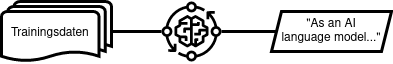
\includegraphics[width=0.7\textwidth]{img/machinelearning_example.png}
        \caption{Primitive Abstraktion eines Modellierungsprozesses für maschinelles Lernen}
        \label{fig:primitive_Abstraktion_eines_Modellierungsprozesses_für_maschinelles_Lernen}
        \vspace{8mm}
    \end{figure}
    
    Der Trainingsprozess erfolgt durch die Optimierung von Modellparametern unter Verwendung von mathematischen Optimierungsmethoden wie dem Gradientenabstieg.
    Durch wiederholtes Training und Feinabstimmung der Modelle können sie kontinuierlich verbessert werden, um präzisere Vorhersagen zu generieren oder überlegene Leistungen bei bestimmten Aufgaben zu erzielen.
    \footfullcite{rebala2019machine}\footfullcite{el2015machine}

\subsection{Deep Learning}

    Deep Learning ist ein Teilbereich des maschinellen Lernens, der sich auf die Nutzung neuronaler Netzwerke mit mehreren Schichten konzentriert.
    Neuronale Netzwerke sind mathematische Modelle, welche biologische Neuronen simulieren und Schichten von verbundenen Neuronen enthalten. Jede Schicht empfängt Eingaben von der vorherigen Schicht und leitet Ausgaben an die nächste Schicht weiter.

    Ein Hauptvorteil des Deep Learnings gegenuber allgemeinerem Maschinellem Lernen, liegt in der automatischen Extraktion von Merkmalen aus den Daten, ohne dass ein Experte diese manuell definieren muss.
    Durch die Kombination mehrerer Schichten können neuronale Netzwerke komplexe Muster und abstrakte Darstellungen erfassen, wodurch sie hochdimensionale Daten effektiv verarbeiten können.
    
    Das Training von Deep-Learning-Modellen erfolgt üblicherweise mit großen Datensätzen und leistungsstarken GPUs, um die erforderlichen Berechnungen effizient durchführen zu können.
    Durch das iterative Training der Netzwerke werden die Gewichtungen und Parameter der einzelnen Neuronen angepasst, um die Fähigkeit des Modells zur präzisen Vorhersage oder Lösung komplexer Aufgaben zu verbessern.
    
    Im weiteren Verlauf werden die grundlegenden Komponenten und Funktionen von Convolutional Neural Networks (CNNs) erläutert, die eine spezielle Art von neuronalen Netzwerken darstellen und insbesondere in der Bildverarbeitung weit verbreitet sind.
    \footfullcite{lecun2015deep}\footfullcite{schmidhuber2015deep}\footfullcite{learning2020deep}

\subsection{Grundlagen von Convolutional Neural Networks}

    Convolutional Neural Networks (CNNs) sind eine spezielle Art von neuronalen Netzwerken, die in der Lage sind, Muster und Merkmale in Bildern effektiv zu erkennen. 
    Sie zeichnen sich durch ihre Fähigkeit aus, lokale Verbindungen und Gewichtungen zwischen den Neuronen herzustellen und so räumliche Informationen in den Daten zu berücksichtigen.
    Die grundlegende Architektur eines CNNs besteht aus mehreren Schichten, darunter Convolutional Layers, Pooling Layers und Fully Connected Layers. 
    In den Convolutional Layers werden Filter verwendet, um lokale Muster und Merkmale zu extrahieren, indem sie über das Eingabebild verschoben werden und die Faltungsoperation durchgeführt wird. 
    Diese Filter können beispielsweise Kanten, Texturen oder spezifische Formen erfassen.
    \begin{wrapfigure}{r}{0.3\textwidth}
        \begin{center}
               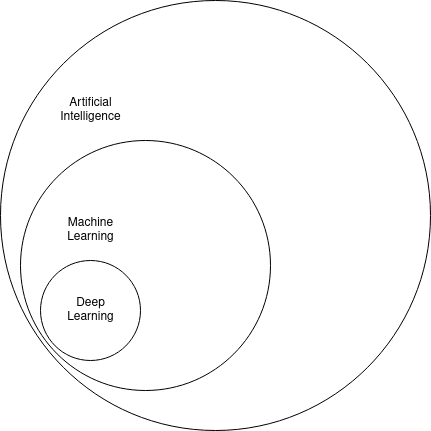
\includegraphics[width=1.06\textwidth]{img/KI-ML-DL.png}
        \end{center}
        \caption{Einordnung der Begriffe Künstliche Intelligenz, Maschine Learning und Deep Learning.}
        \label{fig:KI-ML-DL}
    \end{wrapfigure}

    Nach den Convolutional Layers folgen Pooling Layers, die dazu dienen, die räumliche Dimension der Merkmale zu reduzieren und die wichtigsten Informationen beizubehalten. 
    Typische Pooling-Operationen umfassen das Max-Pooling, bei dem der maximale Wert in einem Bereich ausgewählt wird, und das Average-Pooling, bei dem der Durchschnittswert berechnet wird.
    Die Ausgabe der Pooling Layers wird dann an die Fully Connected Layers weitergeleitet, die eine traditionelle neuronale Netzwerkstruktur aufweisen. Diese Schichten dienen dazu, die erfassten Merkmale zu klassifizieren oder eine Vorhersage zu treffen, indem sie die Gewichtungen der Neuronen anpassen und die Aktivierungsfunktionen anwenden.
    Die Stärke von CNNs liegt in ihrer Fähigkeit, hierarchische Merkmale in den Daten zu erfassen. 
    Die früheren Schichten lernen einfache Merkmale wie Kanten und Ecken, während die späteren Schichten komplexere Merkmale und abstrakte Darstellungen lernen. 
    Durch das Training des Netzwerks mit großen Datensätzen können CNNs die Gewichtungen ihrer Neuronen so anpassen, dass sie die gewünschte Aufgabe, wie beispielsweise die Klassifizierung von Bildern, mit hoher Genauigkeit erfüllen können.
    CNNs haben eine breite Anwendungspalette in der Bildverarbeitung und sind in der Lage, komplexe Aufgaben wie Objekterkennung, Gesichtserkennung, Semantische Segmentierung und Bildgenerierung zu bewältigen. 
    Ihre Leistungsfähigkeit beruht auf der Fähigkeit, automatisch relevante Merkmale aus den Daten zu extrahieren und sie in einer hierarchischen Weise zu verarbeiten.
    In den nächsten Abschnitten werden wir uns genauer mit den einzelnen Komponenten von CNNs befassen, ihre Funktionsweise im Detail untersuchen und verschiedene Architekturen und Techniken kennenlernen, die in der Praxis weit verbreitet sind.
    \footfullcite{lecun1998gradient}\footfullcite{krizhevsky2012imagenet}\footfullcite{simonyan2014very,he2016deep}

    \subsection{Definition und Anwendungen von Convolutional Neural Networks (CNNs)}
    
        Convolutional Neural Networks (CNNs) sind eine Art von künstlichen neuronalen Netzwerken, die speziell für die Verarbeitung von Daten mit räumlicher Struktur entwickelt wurden. 
        Sie zeichnen sich durch ihre Fähigkeit aus, hierarchische Muster und Merkmale in komplexen Daten wie Bildern, Videos oder Tonaufnahmen zu erkennen. 
        CNNs haben in den letzten Jahren enorme Fortschritte in verschiedenen Bereichen der Informatik gemacht, insbesondere in der Bildverarbeitung, Computer Vision und Mustererkennung.
        
        \subsubsection{Einsatz von Convolutional Neural Networks in der Bildverarbeitung}
    
            \acfp{CNN} spielen eine entscheidende Rolle bei der automatischen Analyse und Verarbeitung von visuellen Daten in der Bildverarbeitung. 
            Durch ihre einzigartige Architektur sind sie in der Lage, Bilder in ihre Bestandteile zu zerlegen und räumliche Merkmale wie Kanten, Formen und Texturen zu extrahieren. 
            Dies geschieht durch die Kombination mehrerer Convolutional Layers und Pooling Layers, wodurch komplexe visuelle Muster erlernt und hochdimensionale Daten effektiv verarbeitet werden können. Als Ergebnis haben sich zahlreiche Anwendungen wie Objekterkennung, Gesichtserkennung, semantische Segmentierung und Bildgenerierung entwickelt. 
            Die fortschrittlichen Fähigkeiten von CNNs haben die Leistungsfähigkeit von Bildverarbeitungssystemen erheblich verbessert und zu bahnbrechenden Fortschritten in Bereichen wie autonomes Fahren\footfullcite{huang2020autonomous}, medizinische Bildgebung\footfullcite{boyd2020deep} und Überwachungstechnologie\footfullcite{robbins2022machine} geführt.
        
        \subsubsection{Anwendungen von Convolutional Neural Networks in der Computer Vision}
        
            Die Computer Vision\footfullcite{stockman2001computer} ist ein interdisziplinäres Forschungsfeld, das sich mit der Entwicklung von Algorithmen und Techniken zur Erfassung, Interpretation und Verarbeitung von visuellen Informationen befasst. 
            In diesem Bereich haben \acfp{CNN} eine Revolution ausgelöst (siehe \ref{fig:deeplearning_timeline}), da sie die Fähigkeit besitzen, automatisch relevante visuelle Merkmale aus Bildern oder Videosequenzen zu extrahieren. 
            Durch das Training mit großen Datensätzen können \acp{CNN} lernen, Objekte und Szenen zu erkennen, Gesichter zu identifizieren, Gesten zu verstehen und komplexe visuelle Aufgaben zu lösen. 
            Die Anwendungen von \acp{CNN} in der Computer Vision sind vielfältig und umfassen Bereiche wie automatische Fahrzeugerkennung, Augmented Reality, Robotik und intelligente Überwachungssysteme. 
            Durch den Einsatz von \acp{CNN} wurden die Grenzen der Computer Vision erweitert und Computer sind nun in der Lage, die visuelle Welt um uns herum besser zu verstehen und mit ihr zu interagieren.
        
        \subsubsection{Mustererkennung und Klassifikation mit Convolutional Neural Networks}
    
            Ein weiterer bedeutender Anwendungsbereich von Convolutional Neural Networks (\acfp{CNN}) liegt in der Mustererkennung und Klassifikation. 
            Durch das Training mit annotierten Datensätzen sind \acp{CNN} in der Lage, Muster und Zusammenhänge in den Daten zu erkennen und verschiedene Klassen oder Kategorien von Objekten zu unterscheiden.

            \begin{figure}[h]
                \centering
                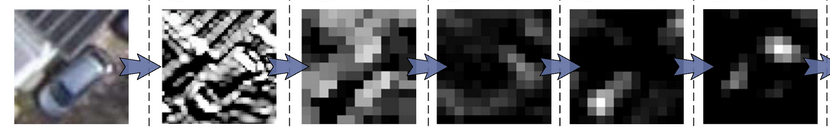
\includegraphics[width=0.7\textwidth]{img/feature_extraction.png}
                \caption{Einsicht in die Vorhergehensweise eines Neuronalen Netzen, und dessen automatische Merkmalsextraktion au mehreren Schichten.\footfullcite{li2018visualizing}}
                \label{fig:feature_extraction}
            \end{figure}
            
            Dies ermöglicht die automatische Klassifizierung von Bildern, Texten, Tonaufnahmen und vielen anderen Datenarten. 
            In den Bereichen der Texterkennung, Spracherkennung, Sprachübersetzung und anderen Bereichen der Mustererkennung haben \acp{CNN} bahnbrechende Fortschritte erzielt. 
            Sie demonstrieren bemerkenswerte Fähigkeiten zur Bewältigung komplexer Klassifikationsaufgaben mit hoher Genauigkeit und haben somit die Effizienz und Genauigkeit von maschinellen Lernsystemen in erheblichem Maße verbessert.
            
        \subsubsection{Weitere Anwendungen}
    
    Neben den oben genannten Bereichen finden Convolutional Neural Networks auch in vielen anderen Bereichen Anwendung. Hier sind einige Beispiele:
    \begin{itemize}
    \item Medizinische Bildgebung: \acp{CNN} werden verwendet, um medizinische Bilder wie Röntgenaufnahmen, MRT-Scans und CT-Scans zu analysieren und Krankheiten zu diagnostizieren. Sie können Tumore, Anomalien oder andere gesundheitliche Zustände identifizieren, was Ärzten bei der genauen Diagnose und Behandlung unterstützt\footfullcite{rahman2020transfer}.

    \item Sprachverarbeitung: \acp{CNN} können in der automatischen Spracherkennung und Sprachsynthese eingesetzt werden. Sie können Audiosignale analysieren und Transkriptionen von gesprochener Sprache generieren. Dies ermöglicht Anwendungen wie Sprachsteuerungssysteme, Sprachassistenten und Untertitelungsdienste.\footfullcite{tandel2020voice}

    \item Finanzanalyse: \acp{CNN} werden zur Vorhersage von Finanzmärkten und zur Erkennung von betrügerischen Transaktionen eingesetzt. Sie können komplexe Muster in historischen Finanzdaten erkennen und Modelle entwickeln, um zukünftige Trends oder Risiken vorherzusagen.\footfullcite{Chen2016finance}

    \item Naturwissenschaften: In den Naturwissenschaften werden \acp{CNN} zur Analyse von großen Datensätzen aus Bereichen wie Astronomie\footfullcite{davies2019using}, Genetik und Teilchenphysik eingesetzt. Sie können dabei helfen, Muster, Zusammenhänge und neue Erkenntnisse in komplexen wissenschaftlichen Daten zu identifizieren. Im Beispiel von Astromoie, können \acp{CNN} eingesetzt werden um seltene Objektiv-Konfigurationen zu finden.

    \end{itemize}
    
    Insgesamt bieten \acfp{CNN} eine vielfältige Bandbreite an Anwendungen, die von der Bildverarbeitung über die Computer Vision bis hin zur Mustererkennung reichen. Ihre Fähigkeit, komplexe Muster in hochdimensionalen Daten zu erfassen, hat die Möglichkeiten der automatisierten Datenverarbeitung und -analyse erweitert und damit zahlreiche innovative Lösungen in verschiedenen Bereichen ermöglicht.
    
\subsection{Wie unterscheiden sich CNNs von anderen neuronalen Netzwerkarchitekturen?}

    \acfp{CNN} stellen eine spezifische Architektur von künstlichen neuronalen Netzwerken dar, die sich in einigen wesentlichen Punkten von anderen Netzwerkarchitekturen unterscheiden. 
    Im Folgenden werden zwei wichtige Unterschiede hervorgehoben:

\subsubsection{Räumlich-sensitive Neuronen und feste Gewichtungen}

    Im Gegensatz zu vollständig verbundenen neuronalen Netzwerken verwenden \acp{CNN} räumlich-sensitive Neuronen und feste Gewichtungen, um lokale Muster in den Eingabedaten zu erkennen. 
    Bei einem vollständig verbundenen Netzwerk sind alle Neuronen einer Schicht mit allen Neuronen der nächsten Schicht verbunden. 
    Dies führt dazu, dass die räumliche Struktur der Daten nicht berücksichtigt wird und das Netzwerk möglicherweise nicht in der Lage ist, lokale Muster und Zusammenhänge effektiv zu erfassen. 
    \acp{CNN} hingegen verwenden sogenannte Filter oder Kernel, die über das Eingabebild verschoben werden, um lokale Merkmale zu extrahieren.

    \begin{figure}[h]
        \centering
        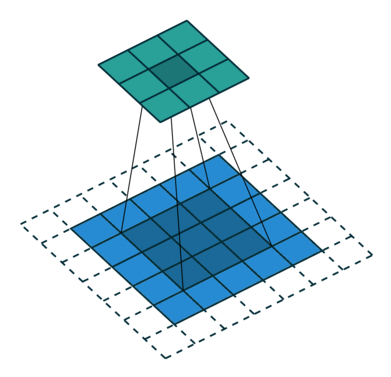
\includegraphics[width=0.4\textwidth]{img/cnn_kernel_sobel.png}
        \caption{Sobel Kernel.}
        \label{fig:cnn_kernel_sobel}
    \end{figure}
    
    Diese Filter\footfullcite{sumangoel151} haben feste Gewichtungen, die während des Trainings angepasst werden, um auf spezifische Muster zu reagieren. 
    Durch die Verwendung räumlich-sensitiver Neuronen und fester Gewichtungen sind \acp{CNN} in der Lage, lokalisierte Merkmale wie Kanten, Texturen und spezifische Formen zu erfassen.

    \subsubsection{Pooling-Operationen zur Dimensionalitätsreduktion und Erhöhung der Robustheit}
    
        Ein weiterer Unterschied besteht darin, dass \acp{CNN} Pooling-Operationen verwenden, um die Dimensionalität der Eingabedaten zu reduzieren und die Robustheit gegenüber Translationen zu erhöhen. 
        Nach den Convolutional Layers folgen in einem CNN typischerweise Pooling Layers. 
        In diesen Schichten werden lokal aggregierte Informationen aus den vorherigen Schichten extrahiert, indem beispielsweise der maximale Wert (Max-Pooling) oder der Durchschnittswert (Average-Pooling) innerhalb eines bestimmten Bereichs ausgewählt wird. 

        \begin{figure}[h]
            \centering
            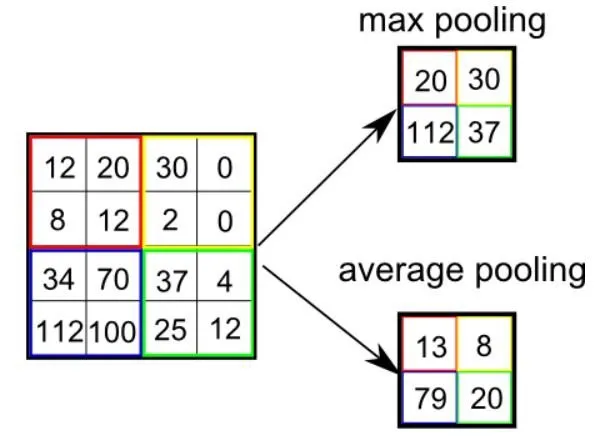
\includegraphics[width=0.4\textwidth]{img/cnn_pooling.png}
            \caption{Max und average Pooling.}
            \label{fig:cnn_kernel_sobel}
        \end{figure}
        
        Durch das Anwenden von Pooling-Operationen wird die räumliche Auflösung der Merkmalskarten reduziert, während wichtige Informationen beibehalten werden. 
        Dies führt zu einer effizienteren Verarbeitung\footfullcite{muhdalifah2022pooling} der Daten und einer erhöhten Robustheit gegenüber kleinen Translationen in den Eingabedaten. 
        Diese Eigenschaft ist besonders vorteilhaft, wenn die genaue Position der Merkmale in den Daten nicht von entscheidender Bedeutung ist.
        Die Verwendung räumlich-sensitiver Neuronen und fester Gewichtungen sowie die Integration von Pooling-Operationen sind charakteristische Merkmale von \acfp{CNN}, die es ihnen ermöglichen, räumliche Informationen zu berücksichtigen, lokale Muster zu erkennen und komplexe visuelle Aufgaben effektiv zu bewältigen.

\subsection{Warum sind Convolutional Neural Networks besonders nützlich für Bild- und Videodaten?}

    \acfp{CNN} haben sich als äußerst nützlich und effektiv bei der Verarbeitung von Bild- und Videodaten erwiesen. Im Folgenden werden einige Gründe dafür erläutert:

\subsubsection{Automatische Merkmalsextraktion}

    \acfp{CNN} haben die Fähigkeit, automatisch Merkmale aus Bildern und Videos zu extrahieren, ohne dass eine manuelle Merkmalsextraktion erforderlich ist. 
    Traditionelle Ansätze zur Verarbeitung von visuellen Daten erforderten oft die Definition und Konstruktion von spezifischen Merkmalsvektoren durch Experten. 
    Im Gegensatz dazu können \acp{CNN} lernen, hierarchische Merkmale direkt aus den Rohdaten zu extrahieren. 
    Durch die Kombination von Faltungs- und Pooling-Schichten sind \acp{CNN} in der Lage, lokale Muster wie Kanten, Texturen und Formen zu erkennen, die zur Identifizierung von Objekten und zur Klassifizierung von Bildern wesentlich sind.
    \footfullcite{ertel2016grundkurs}

\subsubsection{Lernen räumlicher Hierarchien von Merkmalen}

    Die Verwendung von faltenden Schichten ermöglicht es \acp{CNN}, räumliche Hierarchien von Merkmalen zu lernen, was sie besonders effektiv für die Objekterkennung und Klassifizierung macht. 
    Durch die schrittweise Anwendung von Faltung und Pooling in aufeinanderfolgenden Schichten können \acp{CNN} komplexe visuelle Konzepte erfassen. 
    Anfängliche Schichten lernen einfache Merkmale wie Kanten und Farbkontraste, während tiefere Schichten komplexere Merkmale wie Formen, Strukturen und Objekte auf höheren Abstraktionsebenen erkennen können. 
    Diese Hierarchie von Merkmalen ermöglicht es \acp{CNN}, Objekte mit hoher Genauigkeit zu identifizieren und Bilder korrekt zu klassifizieren.

\subsubsection{Anpassung auf weitere Anwendungsbereiche}

    Ein weiterer Vorteil von \acp{CNN} ist ihre Fähigkeit, ohne viel Aufwand und vortrainiertes Wissen auf verschiedene Anwendungsbereiche angepasst zu werden. 
    Ein bereits vortrainiertes \ac{CNN} für die Segmentierung von Menschen kann beispielsweise für die Erkennung von Objekten wiederverwendet werden. 
    Indem man das Netzwerk auf neue Daten feinabstimmt (Fine-Tuning), kann es auf spezifische Aufgaben oder Domänen angepasst werden, ohne von Grund auf neu trainiert werden zu müssen.
    Dies spart Zeit und Ressourcen und ermöglicht es, \acp{CNN} für eine Vielzahl von Bild- und Videodaten-Anwendungen einzusetzen.

\subsubsection{Toleranz gegenüber Translationen, Skalierungen und Verzerrungen}

    \acp{CNN} sind auch in der Lage, Translationen, Skalierungen und Verzerrungen in den Eingabedaten zu tolerieren]\footfullcite{lee2020advo}, was für die Verarbeitung von Bildern und Videos von Vorteil ist. 
    Aufgrund der Verwendung von Faltungsschichten und Pooling-Operationen sind \acp{CNN} invariant gegenüber kleinen räumlichen Verschiebungen in den Eingabedaten. 
    Dies bedeutet, dass ein Objekt, das sich leicht innerhalb eines Bildes bewegt oder skaliert oder verzerrt wird, immer noch von einem CNN erkannt und klassifiziert werden kann. 
    Dies ist besonders vorteilhaft für Anwendungen wie die Objekterkennung in Videos oder die Klassifizierung von Bildern, bei denen die Position, Größe oder Ausrichtung der Objekte variieren können.
    Durch die Toleranz\footfullcite{lee2020advo} (siehe Tabelle \ref{tab:KITTY_vergleich}) gegenüber solchen Variationen wird die Robustheit und Zuverlässigkeit von \acp{CNN} in der Verarbeitung von Bild- und Videodaten verbessert. 
    Sie können auch mit unterschiedlichen Auflösungen von Bildern umgehen und sind in der Lage, Informationen auf verschiedenen Skalenebenen zu extrahieren.
    Diese Fähigkeiten machen \acp{CNN} zu einem effektiven Werkzeug für eine Vielzahl von Bild- und Videodaten-Anwendungen.

    \begin{table}[h]
        \centering
        \begin{tabular}{lcccccccc}
             & \multicolumn{2}{c}{RGB-VO} & \multicolumn{2}{c}{D-VO} & \multicolumn{4}{c}{AD-VO} \\
             & \multicolumn{2}{c}{skip-ordering} & \multicolumn{2}{c}{no skip-ordering} & \multicolumn{2}{c}{skip-ordering} & \multicolumn{2}{c}{no skip-ordering} \\
            Seq & Trans\% & Rot[deg/m] & Trans. & Rot. & Trans. & Rot. & Trans. & Rot. \\
            8 & 14.39 & 0.0452 & 16.41 & 0.0547 & 13.36 & 0.0478 & 9.21 & 0.0341 \\
            9 & 9.59 & 0.0397 & 13.7 & 0.0417 & 8.79 & 0.0365 & 7.43 & 0.032 \\
            10 & 19.18 & 0.0438 & 18.48 & 0.0954 & 14.36 & 0.0671 & 7.26 & 0.0317 \\
            avg & 13.83 & 0.0438 & 16.02 & 0.0562 & 12.44 & 0.0474 & 8.59 & 0.0334 \\
            std & 2.718 & 0.0023 & 1.407 & 0.0147 & 1.995 & 0.0083 & 0.868 & 0.001 \\
        \end{tabular}
        \caption{Leistung der Algorithmen: Translations- und Rotationsfehler von Testsequenzen unter Verwendung des KITTI Devkit. AD-VO funktioniert zuverlässig in verschiedenen Fahrumgebungen. 'D' steht für die Verwendung einer Disparitätskarte und 'A' bedeutet, dass das Modell einen Attention-Block anpasst.}
        \label{tab:KITTY_vergleich}
    \end{table}
    
    
    Von der automatischen Erkennung von Objekten und Gesichtern bis hin zur semantischen Segmentierung und Bildgenerierung haben \acp{CNN} die Grenzen der Bildverarbeitung und Computer Vision erweitert und bahnbrechende Fortschritte in Bereichen wie autonomes Fahren, medizinische Bildgebung und Überwachungstechnologie ermöglicht.
    Insgesamt sind Convolutional Neural Networks aufgrund ihrer automatischen Merkmalsextraktion, des Lernens räumlicher Hierarchien von Merkmalen, der Anpassungsfähigkeit auf verschiedene Anwendungsbereiche und der Toleranz gegenüber Translationen, Skalierungen und Verzerrungen besonders nützlich für die Verarbeitung und Analyse von Bild- und Videodaten.

\section{Anwendungen von CNNs}

	\acfp{CNN} finden in vielen Anwendungsgebieten Anwendung, insbesondere in der Bildverarbeitung und Mustererkennung.
	Durch ihre Fähigkeit, komplexe Merkmale zu erkennen und Bilder automatisch zu klassifizieren, haben sie bahnbrechende Fortschritte in verschiedenen Bereichen erzielt.

\subsection{Bildklassifikation}

    \begin{figure}[h]
        \centering
        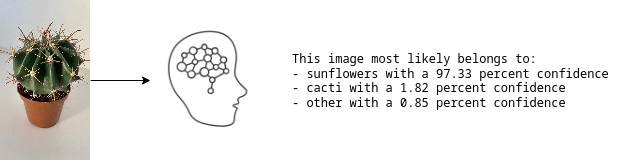
\includegraphics[width=0.7\textwidth]{img/model_sagt_aus.png}
        \caption{Modell zur Bildklassifizierung}
        \label{fig:modell_sagt_aus}
    \end{figure}

    Bildklassifikation ist eine der grundlegenden Anwendungen von \acp{CNN}. 
    Mit Hilfe von trainierten Modellen können \acp{CNN} Bilder automatisch in verschiedene Kategorien klassifizieren, wie beispielsweise Hund vs. Katze, Auto vs. Fahrrad usw. Diese Fähigkeit beruht auf der Nutzung tieferer Schichten in einem CNN. 
    Durch diese tieferen Schichten können komplexe Merkmale wie Texturen, Formen und Strukturen erkannt werden, was zu einer verbesserten Bildklassifikation führt. 
    Indem \acp{CNN} lernen, spezifische Merkmale auf verschiedenen Abstraktionsebenen zu erfassen, können sie komplexe visuelle Muster in Bildern effizient identifizieren und analysieren.
    \footfullcite{guo2017simple}
    
\subsection{Objekterkennung}

    \begin{figure}[h]
        \centering
        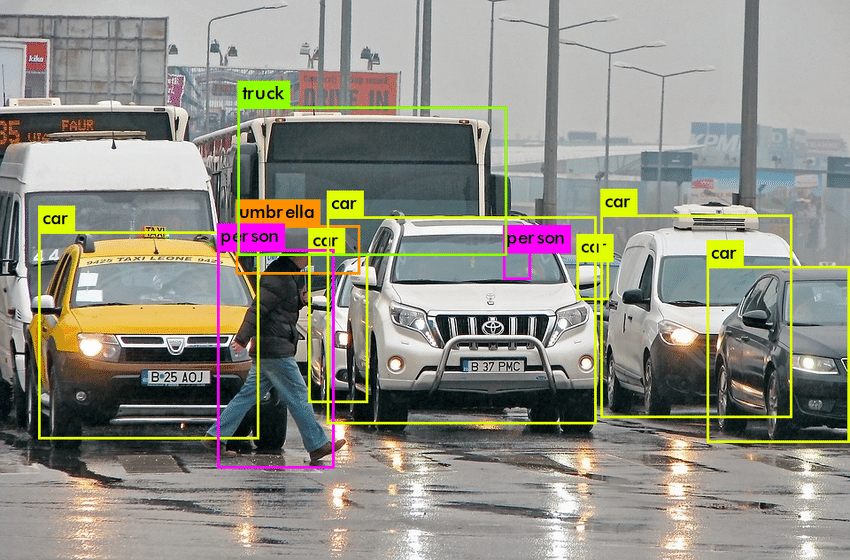
\includegraphics[width=0.4\textwidth]{img/Object-detection-in-a-dense-scene.ppm.png}
        \caption{Modell zur Objekterkennung.}
        \label{fig:modell_finded_etwas}
    \end{figure}

	\acfp{CNN} werden häufig für die Erkennung und Lokalisierung von Objekten in Bildern eingesetzt (siehe Bild \ref{fig:modell_finded_etwas}\footfullcite{Triantafyllidou2017}).
	Durch die Nutzung tieferer Schichten können \acp{CNN} komplexe Merkmale wie Texturen, Formen und Strukturen erkennen, was die Genauigkeit der Bildklassifikation verbessert.
	Zusätzlich ermöglicht der Einsatz von Region Proposal Networks (RPNs) den \acp{CNN}, die genauen Begrenzungsrahmen der erkannten Objekte zu berechnen.

\subsection{Gesichtserkennung}

    \begin{figure}[h]
        \centering
        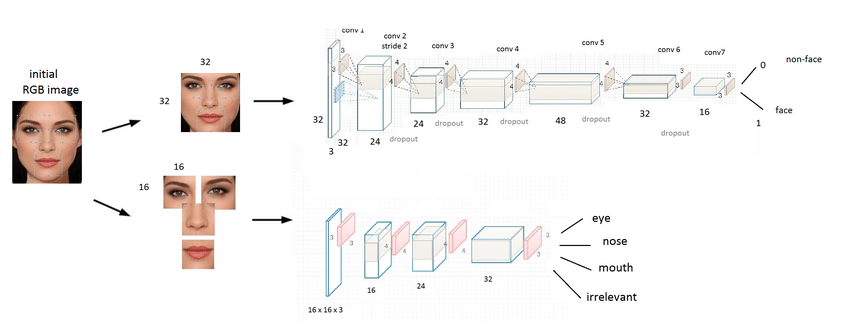
\includegraphics[width=0.8\textwidth]{img/Top-The-CNN-trained-for-the-task-of-full-face-detection-Bottom-The-CNN-trained-for-the.png}
        \caption{Modell zur Gesichtserkennung.}
        \label{fig:modell_finded_gesicht}
    \end{figure}

	\acfp{CNN} haben in der Gesichtserkennung signifikante Fortschritte gemacht und werden häufig für die Identifizierung von Personen in Bildern und Videos eingesetzt.
	Durch den Einsatz von \acp{CNN} können Gesichtsmerkmale wie Augen, Nase und Mund erkannt und zur Identifizierung von Personen verwendet werden.
	Diese Technologie findet Anwendung in Zugangskontrollen, Überwachungssystemen und biometrischer Authentifizierung.

\subsection{Natural Language Processing (NLP)}

	Obwohl \acp{CNN} hauptsächlich für die Verarbeitung von Bildern entwickelt wurden, können sie auch in bestimmten Anwendungen des \acf{NLP} eingesetzt werden\footfullcite{wang2018application}.
	In der \acf{NLP} können \acp{CNN} zur Klassifizierung von Texten, Sentimentanalyse, maschinellen Übersetzung und Textgenerierung eingesetzt werden.
	Durch die Anwendung von Faltungsschichten auf Textsequenzen können \acp{CNN} relevante Merkmale extrahieren und wichtige Informationen für die Klassifizierung liefern.

\subsection{Weitere Anwendungen}

	Neben den oben genannten Anwendungen finden \acp{CNN} in vielen anderen Bereichen Anwendung, wie zum Beispiel in der medizinischen Bildgebung, bei autonomen Fahrzeugen und der Spracherkennung.
	Sie ermöglichen die Automatisierung und Verbesserung verschiedener Aufgaben, indem sie Muster und Zusammenhänge in den Daten erkennen.
	Mit der kontinuierlichen Weiterentwicklung von \acp{CNN} eröffnen sich ständig neue Anwendungsmöglichkeiten in verschiedenen Branchen.

\section{Architektur von CNNs}

\subsection{Input Layer}

    Die Input Layer eines \acfp{CNN} spielt eine entscheidende Rolle bei der Aufnahme und Vorverarbeitung der Rohdaten, die in der Regel Bilder oder Videos sind. 
    Sie ist die erste Schicht des Netzwerks und ermöglicht den Datenfluss in das \ac{CNN}.
    Die Eingabeschicht besteht aus einer Anordnung von Neuronen, wobei jedes Neuron mit einem bestimmten Bereich des Eingabebildes verbunden ist. 

    \begin{figure}[h]
        \centering
        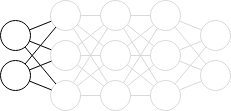
\includegraphics[width=0.5\textwidth]{img/input_layers.png}
        \caption{Input layers}
        \label{fig:input_layers}
    \end{figure}
    
    Diese Verbindungen stellen sicher, dass jedes Neuron Informationen aus einem begrenzten lokalen Bereich des Bildes erhält. Auf diese Weise kann das \ac{CNN} räumliche Informationen über die Daten berücksichtigen und lokalisierte Merkmale erfassen.
    Die Größe der Input Layer ist normalerweise fest vorgegeben, um eine konsistente Verarbeitung der Daten sicherzustellen. 
    Für RGB-Bilder beträgt die typische Größe beispielsweise 244x244x3, wobei die ersten beiden Dimensionen die Breite und Höhe des Bildes repräsentieren und die letzte Dimension die Farbkanäle (Rot, Grün, Blau) darstellt.
    Die Input Layer spielt eine wichtige Rolle bei der Einführung der Daten in das \ac{CNN} und ermöglicht die weitere Verarbeitung und Extraktion von Merkmalen in den nachfolgenden Schichten. 
    Durch die Struktur der Input Layer können CNNs komplexe visuelle Muster in den Daten erkennen und in der Lage sein, komplexe Aufgaben wie Objekterkennung, Gesichtserkennung und Semantische Segmentierung effektiv zu bewältigen.
    \footfullcite{murphy2016overview}

\subsection{Hidden Layers}
    Die Hidden Layers\footfullcite{pyimagesearch} bilden die Hauptkomponente eines \acfp{CNN} und bestehen standardmäßig aus Convolutional-Layern, Pooling-Layern, vollständig verbundenen Layern und Aktivierungsfunktionen. 
    Diese Schichten spielen eine entscheidende Rolle bei der Verarbeitung und Extraktion von Merkmalen aus den Eingabedaten.
    Die Convolutional-Layer führen Faltungsoperationen auf den Eingabedaten durch, um lokale Muster und Merkmale zu extrahieren. Durch die Anwendung von Filtern auf die Eingabedaten werden wichtige Informationen hervorgehoben und irrelevante Details unterdrückt. 
    Dies ermöglicht es dem \ac{CNN}, Merkmale wie Kanten, Texturen und Formen zu erkennen, die für die spätere Klassifizierung oder Segmentierung von entscheidender Bedeutung sind.

    \begin{figure}[h]
        \centering
        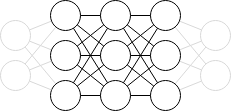
\includegraphics[width=0.4\textwidth]{img/hidden_layers.png}
        \caption{Hidden layers}
        \label{fig:hidden_layers}
    \end{figure}
    
    Die Pooling-Layer sind für die Reduzierung der Dimensionalität der Daten verantwortlich. 
    Sie ermöglichen es, die Größe der Merkmalskarten zu verkleinern und die Anzahl der Parameter im Modell zu reduzieren. 
    Der Hauptzweck des Pooling besteht darin, die Rechenkomplexität des Modells zu verringern, indem weniger Merkmale beibehalten werden. 
    Durch das Zusammenfassen von Informationen wird auch die Lokalisierungsinvarianz verbessert, da die genaue Position eines bestimmten Merkmals in den Merkmalskarten weniger wichtig wird.
    Jedoch erhöhen Pooling-Layer nicht unbedingt die Translationssicherheit. Während des Pooling-Prozesses kann ein gewisser Informationsverlust auftreten, da nur die dominanten Merkmale beibehalten werden. 
    Dadurch können Feinheiten und detaillierte Informationen verloren gehen, die möglicherweise für die genaue Klassifizierung oder Segmentierung von Objekten von Bedeutung sind.
    Insgesamt sind Pooling-Layer eine wichtige Komponente von \acp{CNN}, da sie die Dimensionalität reduzieren und die Rechenressourcen effizienter nutzen können. 
    Es ist jedoch wichtig, sie mit Bedacht einzusetzen, abhängig von den Anforderungen der spezifischen Aufgabe und dem Trade-off zwischen Dimensionsreduktion und dem Erhalt wichtiger Informationen. 
    Die Auswahl der richtigen Pooling-Strategie und -Parameter ist entscheidend, um ein optimales Gleichgewicht zwischen Dimensionalitätsreduktion und Informationsbewahrung zu erreichen.
    \footfullcite{murphy2016overview}

\subsection{Output Layers}
    Die Output Layers bilden die letzte Schicht eines \acfp{CNN} und sind für die Generierung der endgültigen Vorhersage, Klassifizierung oder Segmentierung verantwortlich. 
    Die Ausgabeschicht ist entscheidend für die Interpretation der durch das \ac{CNN} ermittelten Merkmale und ermöglicht die Ausgabe der gewünschten Ergebnisse.
    Ähnlich wie bei den Hidden Layers führen Convolutional-Layer auch in der Ausgabeschicht Faltungsoperationen auf den vorverarbeiteten Eingabedaten durch. 

    \begin{figure}[h]
        \centering
        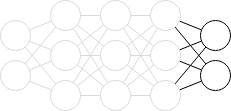
\includegraphics[width=0.5\textwidth]{img/output_layers.png}
        \caption{Output layers}
        \label{fig:output_layers}
    \end{figure}

    Diese Operationen dienen dazu, die relevanten Merkmale zu extrahieren und sie für die weitere Verarbeitung und Interpretation verfügbar zu machen. Die in den vorherigen Schichten erlernten Merkmale werden hier zusammengeführt, um eine aussagekräftige Vorhersage oder Klassifizierung zu ermöglichen.
    Die Form der Ausgabeschicht variiert je nach Anwendungsfall. Bei binärer Klassifizierung besteht die Ausgabeschicht in der Regel aus einem einzelnen Neuron, das eine Wahrscheinlichkeit oder Entscheidung für eine der beiden Klassen ausgibt. 
    Bei Multi-Klassen-Klassifizierung hingegen werden mehrere Neuronenausgaben verwendet, um die Wahrscheinlichkeiten oder Entscheidungen für jede einzelne Klasse zu liefern.
    In unserem spezifischen Projekt ist die Ausgabeschicht ein weiteres Bild, das genau die gleiche Größe wie das Eingangsbild hat. 
    Dies ermöglicht die Segmentierung des Eingangsbildes in verschiedene Bereiche oder die Generierung eines verarbeiteten Ausgabebildes mit spezifischen Eigenschaften.
    Die Ausgabeschicht stellt somit das Endergebnis des CNNs dar und ist entscheidend für die Interpretation und Verwendung der ermittelten Merkmale. 
    Durch eine passende Auswahl der Ausgabeschicht können wir die gewünschten Ergebnisse erzielen, sei es eine Klassifizierung, Segmentierung oder die Generierung eines verarbeiteten Ausgabebildes.

\section{Convolutional layers}

\subsection{Pooling Layers}

    Die Pooling Layers spielen eine wichtige Rolle in der Architektur von \acfp{CNN}. 
    Ihr Hauptzweck besteht darin, die Dimensionalität der Daten zu reduzieren, indem sie die Aktivierungswerte in bestimmten Bereichen zusammenfassen. 
    Dies ermöglicht eine effizientere Verarbeitung der Daten und eine Verbesserung der räumlichen Invarianz gegenüber kleinen Translationen.
    In der Regel werden in CNNs zwei gängige Pooling-Operationen verwendet: das Max-Pooling und das Average-Pooling. 
    Beim Max-Pooling wird der maximale Aktivierungswert in einem bestimmten Bereich ausgewählt und als Ergebnis verwendet. 
    Beim Average-Pooling hingegen wird der Durchschnitt der Aktivierungswerte in diesem Bereich berechnet. 
    Diese Operationen ermöglichen eine Reduktion der Merkmalsdimensionen und helfen dabei, relevante Informationen beizubehalten.

        \begin{figure}[h]
            \centering
            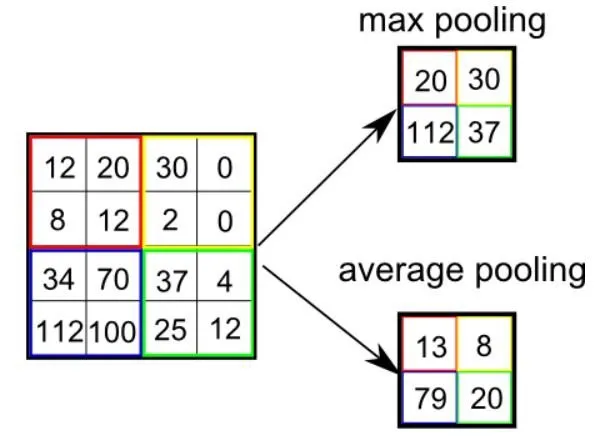
\includegraphics[width=0.4\textwidth]{img/cnn_pooling.png}
            \caption{Max und average Pooling.}
            \label{fig:cnn_kernel_sobel_2}
        \end{figure}
    
    In den meisten \ac{CNN}-Architekturen werden Max-Pooling-Layers eingesetzt, da sie in der Regel bessere Ergebnisse erzielen. 
    Durch die Auswahl des maximalen Aktivierungswerts wird sichergestellt, dass die dominanten Merkmale erhalten bleiben und die Netzwerkperformance verbessert wird.
    Pooling-Schichten bieten auch den Vorteil, die Anzahl der Parameter im Netzwerk zu reduzieren. 
    Durch das Zusammenfassen der Informationen wird die Anzahl der zu lernenden Parameter verringert, was zu einer effizienteren Verarbeitung führt und Overfitting reduzieren kann.
    Ein weiterer Vorteil von Pooling-Layern besteht darin, dass sie die räumliche Invarianz gegenüber kleinen Translationen fördern. Da nur die relevanten Merkmale beibehalten werden, wird die Position dieser Merkmale in den Merkmalskarten weniger wichtig. 
    Dies ermöglicht dem \acp{CNN}, auf ähnliche Merkmale in verschiedenen Bereichen eines Bildes zu reagieren und eine gewisse Robustheit gegenüber Translationen zu erreichen.
    Zusammenfassend kann gesagt werden, dass Pooling Layers eine wichtige Komponente in der Architektur von CNNs sind. 
    Sie helfen dabei, die Dimensionalität zu reduzieren, die Anzahl der Parameter zu verringern und die räumliche Invarianz gegenüber Translationen zu verbessern. 
    Durch die sorgfältige Auswahl und Platzierung von Pooling-Schichten können wir die Effizienz und Leistungsfähigkeit des CNNs steigern.

\subsection{Fully Connected Layers}

    Fully Connected Layers, auch bekannt als vollständig verbundene Schichten, sind traditionelle neuronale Netzwerk-Schichten, bei denen alle Neuronen mit allen Neuronen der vorherigen Schicht verbunden sind.
    Diese Schichten spielen eine wichtige Rolle in der Architektur von \acfp{CNN} und dienen normalerweise am Ende des Netzwerks, um die extrahierten Merkmale zu klassifizieren.   

        \begin{figure}[h]
            \centering
            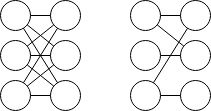
\includegraphics[width=0.5\textwidth]{img/fully_not_connected_layers.png}
            \caption{Links fully conncted, rechts not fully connected layers.}
            \label{fig:fc_layer}
        \end{figure}

    In einem \acp{CNN} werden vor den vollständig verbundenen Schichten in der Regel Convolutional Layers und Pooling Layers verwendet, um Merkmale aus den Eingabedaten zu extrahieren und die Dimensionalität zu reduzieren.
    Diese Merkmale werden dann in den vollständig verbundenen Schichten verwendet, um eine endgültige Klassifizierung oder Vorhersage durchzuführen.    
    Die Anzahl der Neuronen in den vollständig verbundenen Schichten hängt von der Anzahl der Klassen oder der spezifischen Aufgabe ab.
    Wenn beispielsweise ein \acp{CNN} zur Klassifizierung von Bildern in 10 verschiedene Kategorien verwendet wird, wird die Anzahl der Neuronen in der letzten vollständig verbundenen Schicht in der Regel auf 10 festgelegt, um eine Vorhersage für jede Klasse zu ermöglichen.   

\subsection{Overfitting}
        
    Es ist wichtig anzumerken, dass Overfitting ein häufiges Problem in neuronalen Netzwerken ist, insbesondere wenn die Anzahl der Parameter hoch ist.
    Um Overfitting zu minimieren und die Generalisierungsfähigkeit\footfullcite{thanapol2020reducing} des Modells zu verbessern, kann Dropout eingesetzt werden.
    Dropout ist eine Technik, bei der während des Trainings zufällig bestimmte Neuronen und ihre Verbindungen in den vollständig verbundenen Schichten deaktiviert werden.
    Dadurch wird die Vernetzung der Neuronen reduziert und das Modell wird robuster gegenüber Overfitting.

    Data Augmentation ist eine effektive Methode zur Minimierung von Overfitting und Verbesserung der Generalisierungsfähigkeit von Modellen.
    Durch Rotationen können Bilder gedreht werden, um verschiedene Blickwinkel zu simulieren und die Robustheit gegenüber unterschiedlichen Ausrichtungen zu erhöhen.
    Shifting-Techniken ermöglichen das Verschieben von Bildern in verschiedene Richtungen, um die Positionierung der Objekte im Bild zu variieren und die Fähigkeit des Modells zu verbessern, sie unabhängig von ihrer genauen Position zu erkennen.
    Diese Transformationen helfen dabei, mehr Vielfalt in die Trainingsdaten einzuführen und das Modell darauf vorzubereiten, mit verschiedenen Blickwinkeln, Positionen und Perspektiven umzugehen, wodurch die Gefahr von Overfitting verringert und die Fähigkeit zur Generalisierung gesteigert wird.

    \begin{figure}[h]
        \centering
        \begin{minipage}[t]{0.45\textwidth}
            \centering
            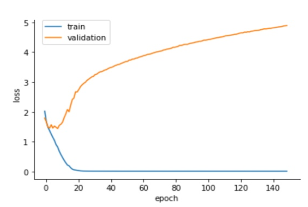
\includegraphics[width=\textwidth]{img/overfitting.png}
            \caption{Overfitting und geringe Generalisierung in alleinigen CNN.}
        \end{minipage}\hfill
        \begin{minipage}[t]{0.45\textwidth}
            \centering
            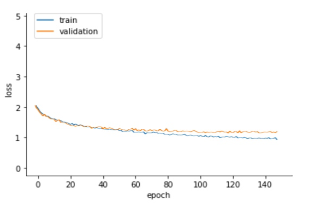
\includegraphics[width=\textwidth]{img/overfitting_mit_data_agumentation_und_shifting_plus_dropout.png}
            \caption{Reduktion von Overfitting und Verbesserung der Generalisierung durch Anwendung von Verschiebung in Breite und Höhe zusammen mit Dropout bei Convolutional Neural Networks (CNN)}
        \end{minipage}
    \end{figure}
    
    Zusammenfassend sind Fully Connected Layers ein wesentlicher Bestandteil der Architektur von CNNs. Sie ermöglichen die Klassifizierung der extrahierten Merkmale und spielen eine entscheidende Rolle bei der Ausführung verschiedener Aufgaben. Die Anzahl der Neuronen in den vollständig verbundenen Schichten wird entsprechend der spezifischen Anforderungen der Aufgabe festgelegt. Durch den Einsatz von Techniken wie Dropout kann das Modell vor Overfitting geschützt werden und eine verbesserte Generalisierungsfähigkeit erzielen.

\subsection{Aktivierungsfunktionen}

    Aktivierungsfunktionen spielen eine wichtige Rolle in der Architektur von \acfp{CNN}. 
    Sie werden auf die Ausgaben der Neuronen angewendet und führen nichtlineare Transformationen durch\footfullcite{Hao2020}. 
    Diese Funktionen ermöglichen es dem Netzwerk, komplexe Zusammenhänge zu modellieren und eine höhere Ausdrucksfähigkeit zu erreichen.    
    In CNNs werden verschiedene Aktivierungsfunktionen verwendet, von denen einige besonders häufig anzutreffen sind. 

    \begin{figure}[h]
        \centering
        \begin{minipage}[t]{0.45\textwidth}
            \centering
            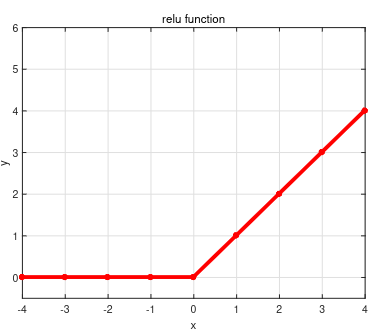
\includegraphics[width=\textwidth]{img/relu_fun.png}
            \caption{ReLu Aktivierungsfunktion.}
        \end{minipage}\hfill
        \begin{minipage}[t]{0.45\textwidth}
            \centering
            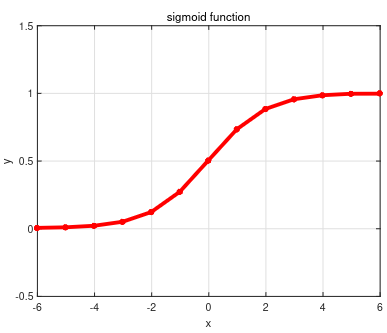
\includegraphics[width=\textwidth]{img/sigmoid_fun.png}
            \caption{Sigmoid Aktivierungsfunktion.}
        \end{minipage}
    \end{figure}

    Eine gängige Aktivierungsfunktion ist die ReLU\footfullcite{wang2020influence} (Rectified Linear Unit), die für positive Eingaben den Wert beibehält und negative Eingaben auf Null setzt. 
    Die ReLU-Funktion ist bekannt für ihre Einfachheit und Effektivität bei der Behandlung von Vanishing-Gradient-Problemen, bei denen die Gradienten während des Trainings verschwinden können.

    Eine weitere gängige Aktivierungsfunktion ist die Sigmoid-Funktion\footfullcite{wang2020influence}, die eine S-förmige Kurve erzeugt. 
    Sie komprimiert den Wertebereich der Ausgabe auf den Bereich zwischen 0 und 1, wodurch die Funktion gut zur Modellierung von Wahrscheinlichkeiten geeignet ist. 
    Die Sigmoid-Funktion wird oft in binären Klassifizierungsaufgaben verwendet.    
    Die tanh-Funktion (Hyperbolic Tangent) ist eine weitere Aktivierungsfunktion, die eine S-förmige Kurve erzeugt, aber im Vergleich zur Sigmoid-Funktion eine symmetrische Ausgabe mit einem Wertebereich zwischen -1 und 1 liefert. 
    Die tanh-Funktion wird oft in mehrklassigen Klassifizierungsaufgaben eingesetzt.    
    Die Verwendung von Aktivierungsfunktionen ermöglicht es \acp{CNN}, nichtlineare Zusammenhänge zu erlernen und komplexe Muster in den Daten zu erkennen. 
    Durch die Einführung von Nichtlinearität können \acp{CNN} flexibler auf verschiedene Eingabemuster reagieren und ihre Fähigkeit zur Modellierung komplexer Zusammenhänge verbessern.    
    Zusammenfassend spielen Aktivierungsfunktionen eine wesentliche Rolle in der Architektur von \acp{CNN}. 
    Sie ermöglichen nichtlineare Transformationen der Neuronausgaben und helfen dabei, die Fähigkeit des Netzwerks zur Modellierung komplexer Zusammenhänge zu verbessern. 
    Die Auswahl der geeigneten Aktivierungsfunktion hängt von der Art der Aufgabe und den spezifischen Anforderungen des Modells ab.

\subsection{Verlustfunktionen}

    Verlustfunktionen sind ein wesentlicher Bestandteil der Architektur von \acfp{CNN}. 
    Sie dienen dazu, den Unterschied zwischen den Vorhersagen des Modells und den tatsächlichen Werten der Daten zu messen. 
    Die Wahl einer geeigneten Verlustfunktion ist entscheidend, um das \ac{CNN} für die spezifische Aufgabe zu optimieren und die Genauigkeit der Vorhersagen zu verbessern\footfullcite{zhu2019new}.
    In der Klassifizierung werden häufig Verlustfunktionen wie die Cross-Entropy-Loss-Funktion verwendet. 
    Diese Funktion misst den Abstand zwischen den Vorhersagen des Modells und den tatsächlichen Klassenlabels der Daten. Sie wird häufig in Multi-Klassen-Klassifizierungsaufgaben eingesetzt und ermöglicht es dem Netzwerk, die Wahrscheinlichkeiten für jede Klasse zu modellieren und den Fehler basierend auf den Abweichungen von den richtigen Klassenlabels zu berechnen.

        \begin{figure}[h]
            \centering
            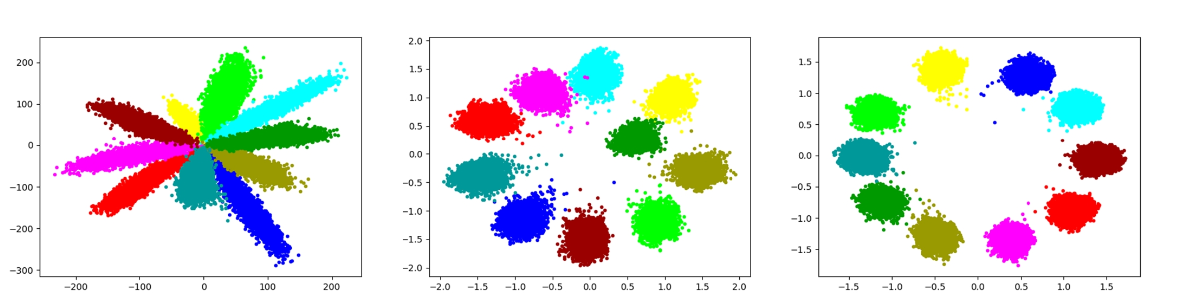
\includegraphics[width=0.8\textwidth]{img/loss_functions.png}
            \caption{Links Softmax-2D, mittig Center-Loss, rechts PEDCC-loss.}
            \label{fig:loss_functions}
        \end{figure}
    
    Die Verlustfunktionen dienen als Grundlage für die Berechnung des Fehlersignals und die Aktualisierung der Gewichte im Netzwerk während des Trainingsprozesses. Durch die Minimierung der Verlustfunktion kann das \ac{CNN} lernen, die optimalen Gewichtungen zu finden und die Genauigkeit der Vorhersagen zu verbessern.
    Es ist wichtig zu beachten, dass die Wahl der Verlustfunktion von der spezifischen Aufgabe abhängt. 
    In einigen Fällen können andere Verlustfunktionen wie die Mean Squared Error (MSE) oder die Binary Cross-Entropy verwendet werden, je nach den Anforderungen der Aufgabe und der Art der Daten.

\begin{lstlisting}[caption={Trainingsverlustverlauf: Unsere Loss-Funktion nimmt kontinuierlich ab, was auf eine verbesserte Modellleistung hinweist.}]
Training [   0/10000] ..........0 )    Loss= 1.1146412
Training [   1/10000] ..........1 )    Loss= 1.0547378
Training [   2/10000] ..........2 )    Loss= 1.1281569

Training [7078/10000] ..........7078 ) Loss= 0.073117875
Training [7079/10000] ..........7079 ) Loss= 0.05900609
Training [7080/10000] ..........7080 ) Loss= 0.040167235
\end{lstlisting}

    Die Verlustfunktionen spielen eine zentrale Rolle in der Architektur von \acp{CNN}, da sie den Unterschied zwischen den Vorhersagen und den tatsächlichen Werten der Daten messen. 
    Sie dienen als Leitfaden für die Optimierung des Modells während des Trainingsprozesses und helfen dabei, die Genauigkeit der Vorhersagen zu verbessern. 
    Die Auswahl der richtigen Verlustfunktion ist entscheidend, um die Leistung des \acp{CNN} zu maximieren und die gestellte Aufgabe erfolgreich zu lösen.
    Indem wir die Architektur und die verschiedenen Schichten eines Convolutional Neural Networks verstehen, können wir die Funktionsweise und die Fähigkeiten dieser leistungsstarken neuronalen Netzwerkarchitektur besser erfassen. 
    \footfullcite{janocha2017loss}\footfullcite{gu2018recent}
    

